% !TEX root=../presentation_1.tex
\section{Background}

\subsection{Basic Assumptions}

\begin{frame}
\frametitle{Basic Assumptions}
\begin{itemize}
\item Synchronous CONGEST model.
\begin{itemize}
    \item \textbf{Synchronous} message-passing model.
    \item Every message is $O(\log n)$ in length.
\end{itemize}
\item In the beginning, every vertex $v$ knows its own \textbf{unique} ID.
\item MST is \textbf{unique}
\begin{itemize}
    \item Without loss of generality, we can assume that MST is unique.
    \item If not, we can always break the symmetry by encode the weights with fractions to be a function of node ID.
\end{itemize}
\end{itemize}
\end{frame}

\begin{frame}
\frametitle{Spanning tree forest}
\begin{figure}
\centering
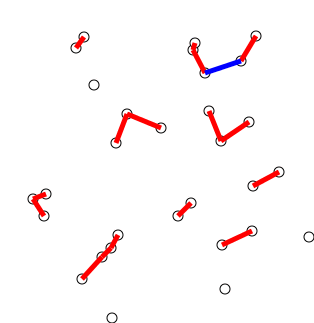
\includegraphics[width=0.5\textwidth]{figures/KruskalDemo-36.png}
\caption{A spanning tree forest}
\end{figure}
\end{frame}

\subsection{Summary of methods}
\begin{frame}
\frametitle{Summary of methods}

\begin{itemize}
    \item $n=|V|, m=|E|.$
    \item $D:$ Hop-diameter of the graph. $D=\max_{u,v \in V} dist(u, v)$.
\end{itemize}
% !TEX root=../presentation_1.tex
\begin{table}
\renewcommand{\arraystretch}{1.3}
\caption{Summary of the complexity of distributed MST algorithms}
\begin{tabular}{|c|c|c|}
\hline
Method         & Time Complexity            & Message Complexity\\
\hline
\hline
Pipeline-MST   & $O(D + n)$                 & $O(m + n^2)$\\
\hline
GHS            & $O(n \log n)$              & $O(m + n \log n)$\\
\hline
Controlled-GHS & $O(D + \sqrt{n} \log^* n)$ & $O(m + n^{\frac{3}{2}})$\\
\hline
\textbf{This Work}& $O((D + \sqrt{n}) \log n)$  & $O(m \log n + n \log n \log^* n)$ \\
\hline
\hline
Randomized [PRS16]& $\tilde{O}(D + \sqrt{n})$  & $\tilde{O}(m)$ \\
\hline
Lower Bound [PRS16] & $\tilde{\Omega}(D + \sqrt{n})$  & $\Omega(m)$ \\
\hline
\end{tabular}
\end{table}

\end{frame}

\subsection{Pipeline-MST}
\begin{frame}
\frametitle{Pipeline-MST}
\begin{itemize}
    \item A distributed version of Kruskal's algorithm.
    \item Build a BFS tree first, $O(D)$ rounds with $O(m)$ messages.
    \item Each node keeps a candidate set, initializes at neighbor edges.
    \item For each round
    \begin{itemize}
        \item Add the incoming edges to the set.
        \item Remove the \textbf{heaviest} edge in any \textbf{cycle} in the set.
        \item Send the \textbf{lightest} candidate to its BFS parent.
    \end{itemize}
    \item After $(D+n-2)$ rounds, the root broadcast the MST edges to the whole tree.
    \item $(D-1)$ rounds to establish stable links between the leaves and the root, and only need $(n-1)$ rounds to find the edges needed for an MST. Use another $(D+n-2)$ rounds to braodcast.
    \item $O(m)$ messages to build BFS tree. Each node sends at most $n$ edges in total.
    \item $O(D+n)$ rounds and $O(m + n^2)$ messages.
\end{itemize}
\end{frame}

\subsection{GHS [GHS86]}
\begin{frame}
\frametitle{GHS Algorithm}
\begin{itemize}
    \item A distributed version of \textbf{Boruvka's} algorithm: merging components.
    \item Each node starts as \textbf{a component tree} with height 0.
    \item At phase $i$, any component with size less than $2^i$ fuses into another MST.
    \item Choose the minimum outgoing edge (MWOE) of each component for merging.
    \item In the worst case, a component may need to wait for $O(n)$ rounds in each phase since the component size can grow to size $O(n)$ in the beginning. 
\end{itemize}
\end{frame}

\subsection{GHS [GHS86]}
\begin{frame}
\frametitle{GHS Algorithm}
\begin{itemize}
    \item Each edge can only be accepted or declined once $O(m)$. Every round each node needs to send convergecast and broadcast once, $O(n \log n)$.
    \item $\log n$ phases, $O(n \log n)$ rounds and $O(m + n \log n)$ messages.
\end{itemize}
\end{frame}

% \subsection{Cole-Vishkin [CV86]}
% \begin{frame}
% \frametitle{Cole-Vishkin's vectex coloring algorithm [CV86]}
% \begin{itemize}
%     \item To further improve the complexity, we need to look at some backgrounds graph vertex coloring.
%     \item In a valid coloring, neighboring vertices have different colors.
%     \item Here, we focus on a graph that is a directed list or a cycle.
%     \item We can always reduce 1 color at a time, until the graph is 3-colored.
%     \item 2-coloring the graph is possible but involves global knowledge.
% \end{itemize}
% \begin{figure}
%     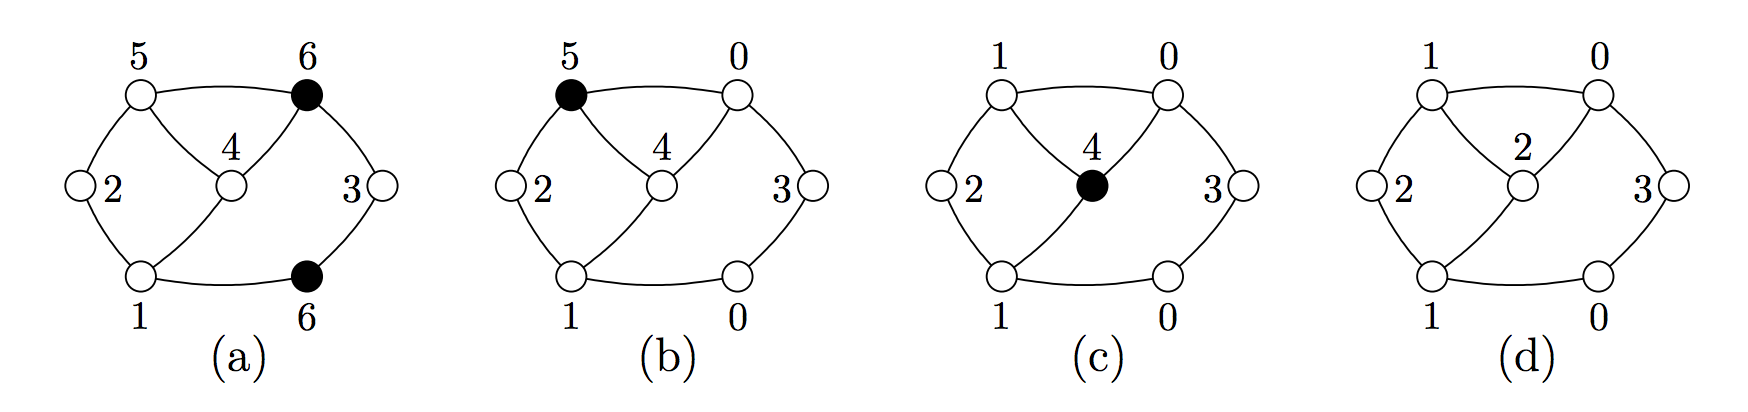
\includegraphics[width=0.9\textwidth]{figures/reduce_one.png}
% \end{figure}
% \end{frame}

% \begin{frame}
% \frametitle{Cole-Vishkin's vectex coloring algorithm [CV86]}
% \begin{figure}
%     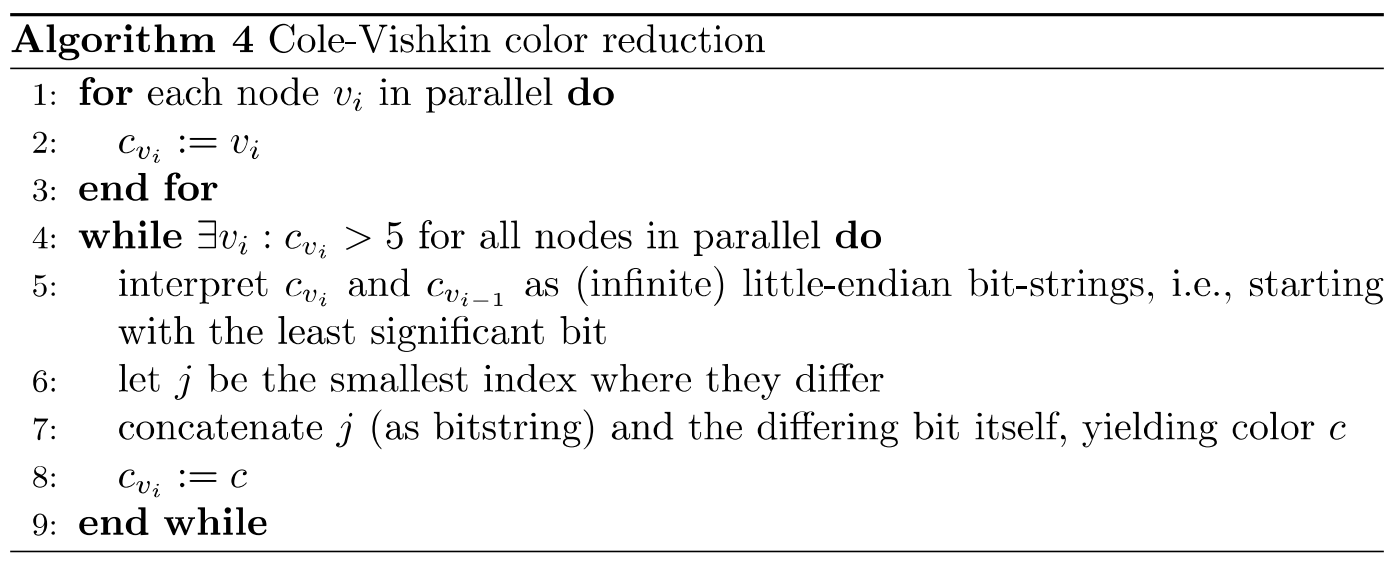
\includegraphics[width=0.9\textwidth]{figures/cole-vishkin.png}
% \end{figure}
% \end{frame}

% \begin{frame}
% \frametitle{Cole-Vishkin's vectex coloring algorithm [CV86]}
% \begin{figure}
%     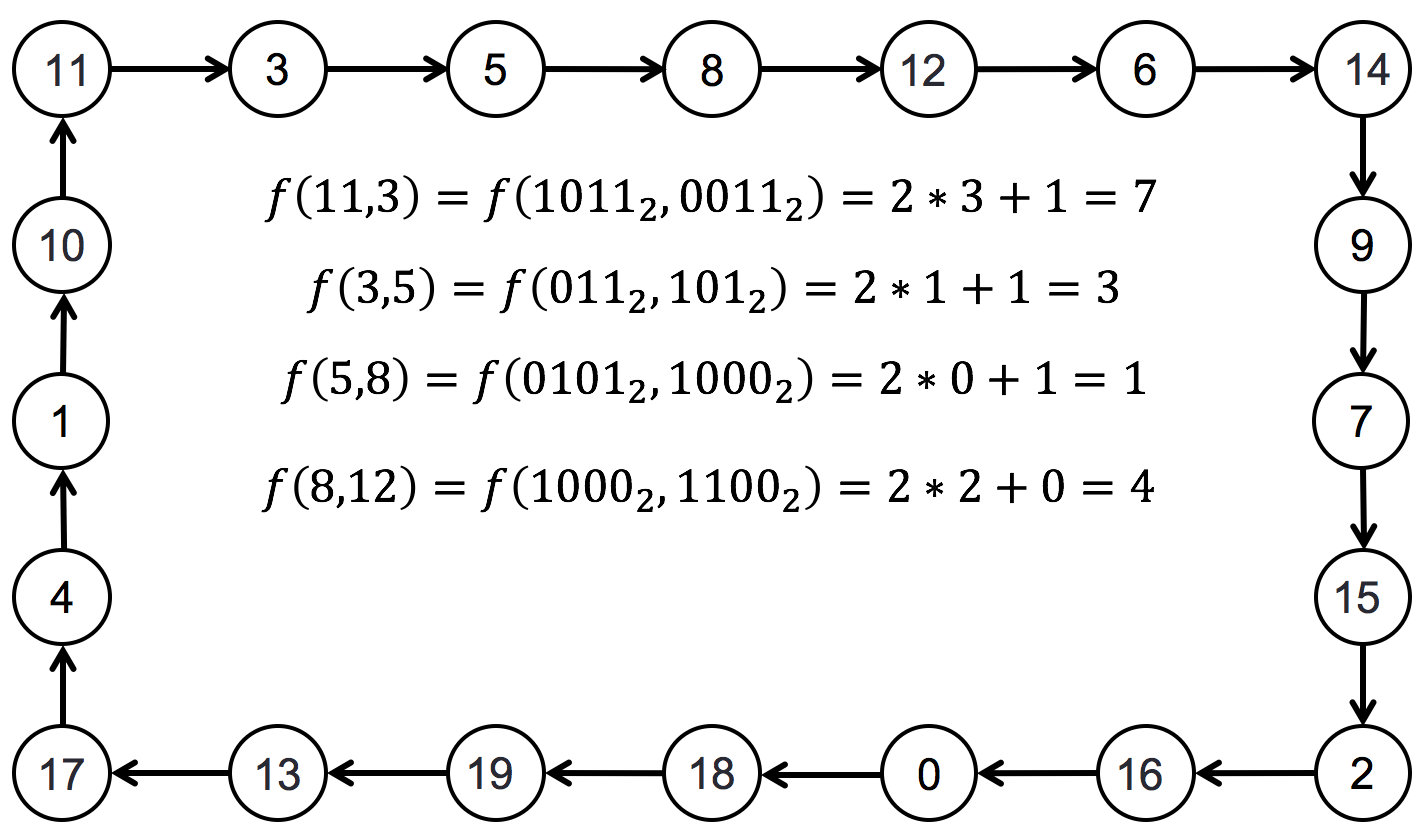
\includegraphics[width=0.9\textwidth]{figures/cole-vishkin-1.png}
% \end{figure}
% \end{frame}

% \begin{frame}
% \frametitle{Cole-Vishkin's vectex coloring algorithm [CV86]}
% \begin{figure}
%     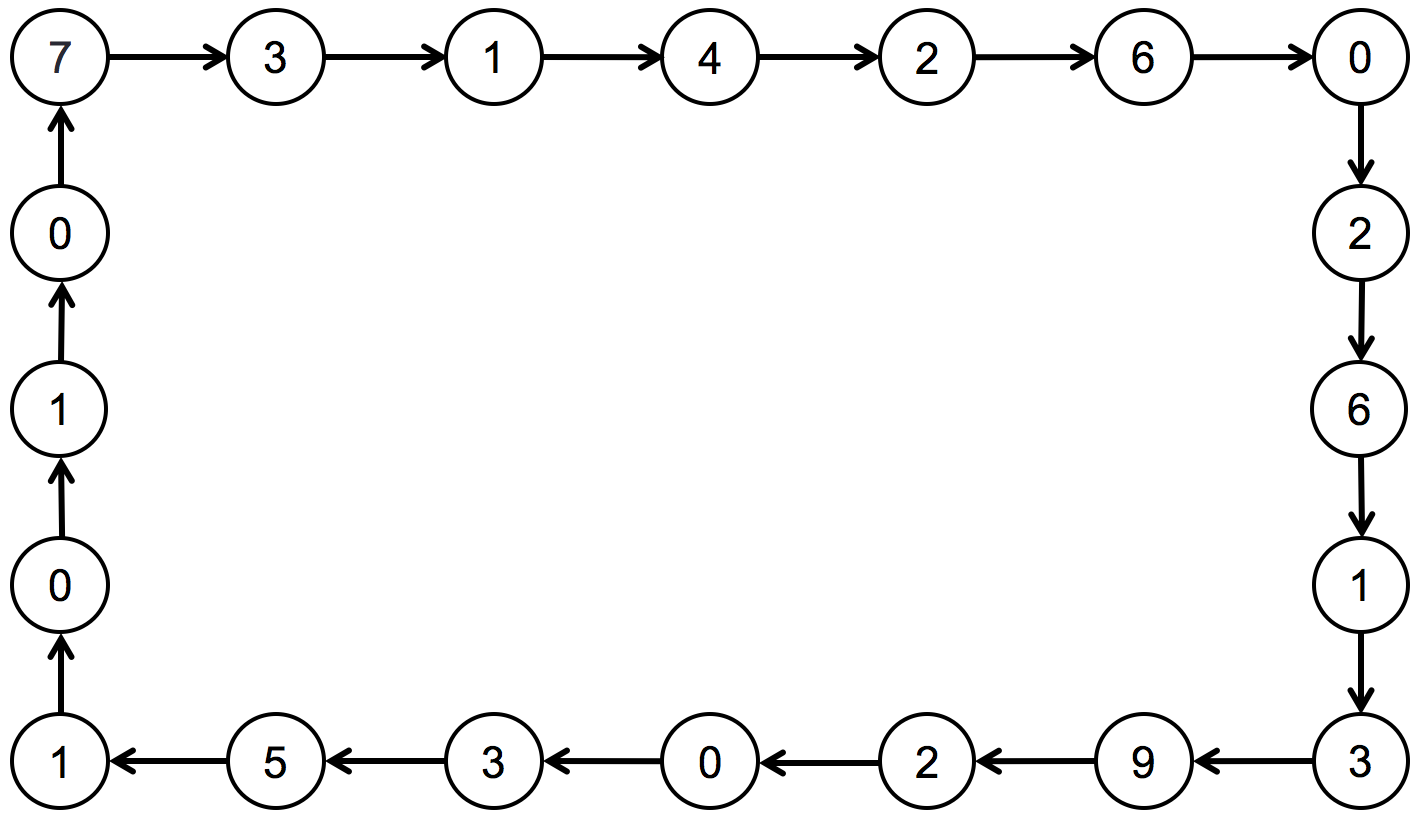
\includegraphics[width=0.9\textwidth]{figures/cole-vishkin-2.png}
% \end{figure}
% \end{frame}

% \begin{frame}
% \frametitle{Cole-Vishkin's vectex coloring algorithm [CV86]}
% \begin{figure}
%     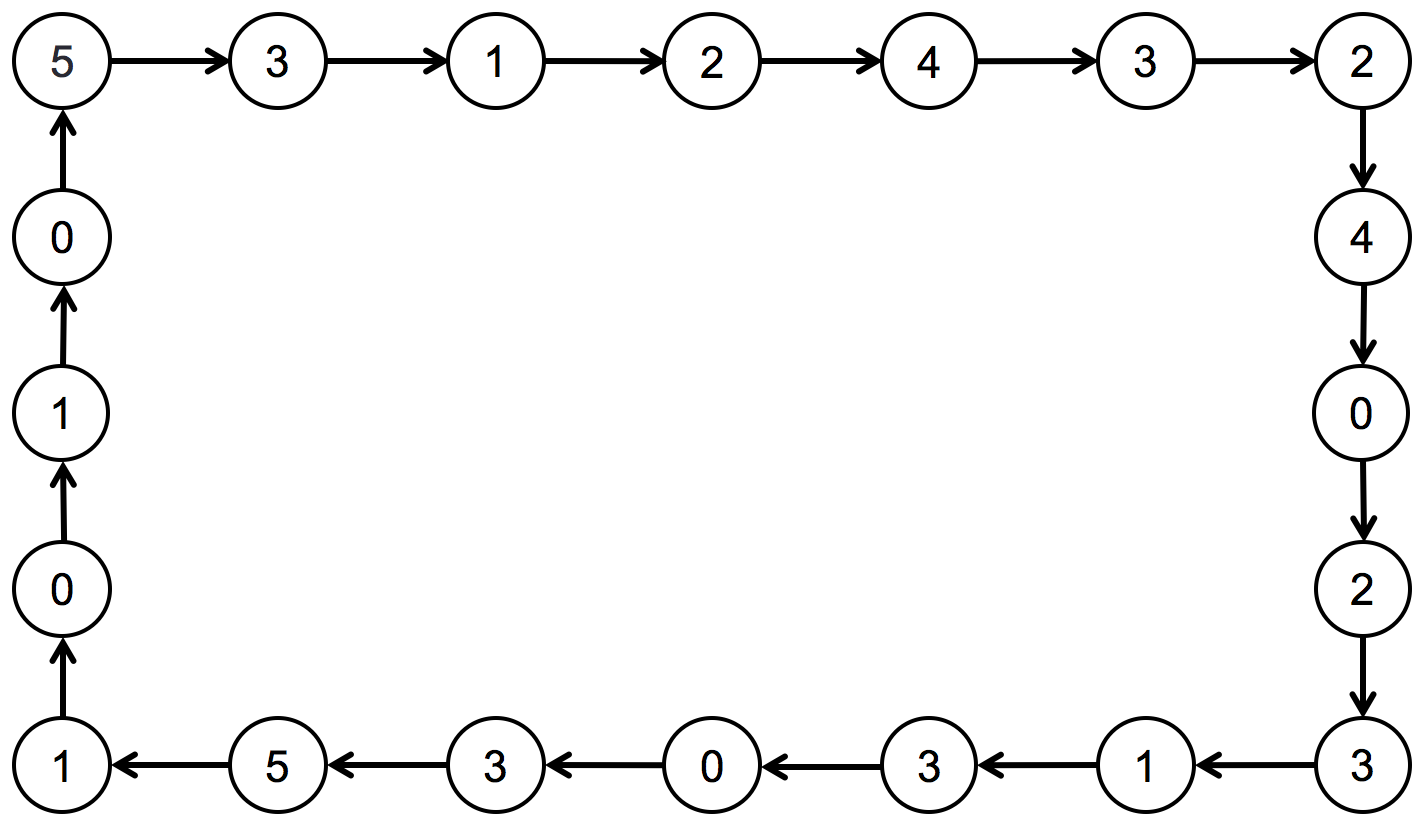
\includegraphics[width=0.9\textwidth]{figures/cole-vishkin-3.png}
% \end{figure}
% \end{frame}

% \begin{frame}
% \frametitle{Cole-Vishkin's vectex coloring algorithm [CV86]}
% \begin{itemize}
%     \item This can bring us a 6-coloring of the graph in $\log^* n$ time ($\log^* 2^{65536} = 5$).
%     \item We can get a 3-coloring by running the naive algorithm for 3 more iterations.
% \end{itemize}
% \end{frame}

% \subsection{Maximal Indepedent Set (MIS) of Rooted Trees [GPS87]}
% \begin{frame}
% \frametitle{Maximal Indepedent Set (MIS) of Rooted Trees [GPS87]}
% \begin{itemize}
%     \item A rooted tree is a tree where edges are directed from children to parents.
%     \item It turns out we can compute a maximal independent set very efficiently on rooted trees.
%     \item We can apply Cole-Vishkin on 3-coloring the rooted tree, just treat each path towards the root as indepedent lists.
%     \item After obtaining a 3-coloring, we can iterate over the colors.
%     \item For each color, a node with that color adds itself to the IS.
%     \item The node also sends a reject message to all of its neighbors, so they will be removed.
%     \item The rejected neighbor can respond to one of the node so that we can get a maximal matching for free.
% \end{itemize}
% \end{frame}

\subsection{Controlled-GHS [GKP98, KP98]}
\begin{frame}
\frametitle{Controlled-GHS Algorithm [GKP98, KP98]}
\begin{itemize}
    \item Pipeline-MST reduces the number of components by 1 per round.
    \item GHS reduces the number of components by half, but trickier merging two giant trees.
    \item Why not combine the two algorithms?
    \item In the first phase, use GHS to reduce the number of components to $\sqrt{n}$. Use maximal matching in the components tree.
    \item Maximal matching on graph: $\log^*(n)$
    \item In the second phase, use Pipeline-MST to reduce the number of components 1 at a time 
    using an auxillary BFS tree.
\end{itemize}
\end{frame}

\begin{frame}
\frametitle{Controlled-GHS Algorithm [GKP98, KP98]}
\begin{itemize}
\item There are $\log \sqrt{n}$ phases.
\item In each phase $i$, we first need to compute the MIS on the minimum-weight outgoing edge (MWOE) of each component. Each takes $O(2^i \log^*n)$ (messages need to traverse at node level). 
\item Then takes $O(2^i)$ to broadcast within the component. So the complexity is dominated by vertex coloring.
\item Therefore the first phase takes $\sum_{i=0}^{\log \sqrt{n}} O(2^i \log^* n) = O(\sqrt{n}\log^*n)$ rounds.
\item The second phase, there are at most $\sqrt{n}$ components left. It takes $O(D + \sqrt{n})$ rounds to finish, since we only need to find $\sqrt{n}$ edges.
\item In total, Controlled-GHS takes $O(D + \sqrt{n}\log^* n)$ rounds, which is time-optimal.
\end{itemize}
\end{frame}

\begin{frame}
\frametitle{Controlled-GHS Algorithm [GKP98, KP98]}
\begin{itemize}
\item However, this algorithm still has a high message complexity.
\item In the first phase, we have $\log \sqrt n$ rounds. 
\item Based on previous analysis, $O(m + n \log \sqrt{n}) = O(m + n\log n)$ messages.
\item In the second phase, it takes $O(m)$ to build a BFS tree. Each node sends at most $\sqrt{n}$ edges in total. 
\item The total message complexity is $O(m+n^{\frac{3}{2}}).$
\end{itemize}
\end{frame}